\documentclass[11pt]{article}

\usepackage{times}
\usepackage[utf8]{inputenc} % allow utf-8 input
\usepackage[T1]{fontenc}    % use 8-bit T1 fonts
\usepackage{url}            % simple URL typesetting
\usepackage{graphics}
\usepackage{color}
\usepackage{amsfonts}       % blackboard math symbols
\usepackage{amsmath}       % blackboard math symbols
\usepackage{amssymb}

\usepackage{lipsum}

\usepackage{tikz}
\usetikzlibrary{angles,quotes,calc}

\usepackage{geometry}
\geometry{left=2.8cm,right=2.8cm,top=2.6cm,bottom=2.6cm}
\usepackage{fancyhdr}
\pagestyle{fancy}
\usepackage{hyperref}% should be the last package you include

\newcommand{\theteam}{}
\newcommand{\team}[1]{\def\theteam{#1}}


\fancyhead[L]{\theteam}
\fancyhead[R]{\thepage}
\cfoot{}

\setlength{\parindent}{0pt}

\team{WayneGradientzky: Rajinish Aneel Bhatia, Bartol Markovinović, Mohd Khizir Siddiqui}
\title{RL-Course 2025/26: Final Project Report}
\author{\theteam}

\begin{document}
\maketitle

\section{Introduction}\label{sec:intro}

\section{Twin Delayed Deep Deterministic Policy Gradient (TD3)}

Twin Delayed Deep Deterministic Policy Gradient (TD3)~\cite{fujimoto2018:TD3} is a 
model-free, off-policy algorithm for continuous action spaces, improving over DDPG via 
clipped double Q-learning, delayed policy updates, and target policy smoothing. TD3 
maintains two Q-networks ($Q_{\phi_1}$ and $Q_{\phi_2}$) and uses their minimum as the 
TD target:
%
\[ y = r + \gamma \min_{i=1,2} Q_{\phi_{i}'}(s', \tilde{a}), \quad
   \tilde{a} = \pi_{\theta'}(s') + \epsilon, \quad 
   \epsilon \sim \texttt{clip}(\mathcal{N}(0,\sigma), -c, c) \]
%
Each critic minimizes the squared Bellman error 
$\mathcal{L}(\phi_i) = \mathbb{E}_{(s,a,r,s')\sim\mathcal{D}}(Q_{\phi_i}(s,a)-y)^2$, 
while the actor maximizes $J(\theta) = \mathbb{E}_{s\sim\mathcal{D}} 
Q_{\phi_1}(s,\pi_\theta(s))$ and is updated every 2 critic steps.

\subsection{Method}
\subsubsection{N-Step Returns}

Instead of the standard one-step TD target, we use $n$-step returns to propagate reward 
signal faster:
%
\[ y = r(s_0) + \gamma r(s_1) + \dots + \gamma^{n-1}r(s_{n-1}) + \gamma^n q(s_n, \tilde{a}) \]

\subsubsection{Custom Opponent and Bank-Shot Reward}

We noticed early on that the model did not always manage to learn ricochet (bank) shots, so to help it defend against opponents that hit those shots we introdued a hard-coded opponent that always plays them.
Given puck position $P$, goal position $G$, and $T$ as the target we must shoot at to reach $G$. Then $T_y$ is known because that is the boundary and we only need to find $T_x$. We can assume that $T_x \ge P_x$ and $G_x \ge T_x$. If we assume frictionless walls than $\theta$ = $\phi$.

\begin{center}
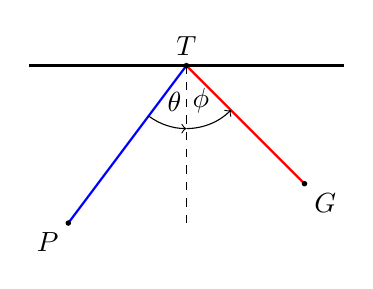
\begin{tikzpicture}[scale=0.5]
  \coordinate (P) at (-3,-2);
  \coordinate (G) at (3,-1);
  \coordinate (T) at (0,2);
  \coordinate (W1) at (-4,2);
  \coordinate (W2) at (4,2);
  \coordinate (N) at (0,-2);
  \draw[thick] (W1) -- (W2);
  \draw[thick, blue] (P) -- (T);
  \draw[thick, red]  (T) -- (G);
  \draw[dashed] (T) -- (N);
  \fill (P) circle (2pt) node[below left]  {$P$};
  \fill (G) circle (2pt) node[below right] {$G$};
  \fill (T) circle (2pt) node[above]       {$T$};
  \pic[draw, ->, angle radius=0.8cm, "$\theta$"]{angle = P--T--N};
  \pic[draw, ->, angle radius=0.8cm, "$\phi$"]  {angle = N--T--G};
\end{tikzpicture}
\end{center}

From $\tan\theta = \tan\phi$ we obtain:
%
\[ T_x = \frac{|T_y - P_y|\,G_x + |T_y - G_y|\,P_x}{|T_y - G_y| + |T_y - P_y|} \]
%
This agent achieves ${\approx}94\%$ win rate against the weak opponent and ${\approx}80\%$ 
against the strong opponent. We also shaped the reward by calculating how aligned the agent's direction was to this direction to encourage the learning agent to prefer shots in this direction.

\subsubsection{Layer Normalization}

\textbf{Layer Normalization.} Layer normalization normalizes activations across the feature dimension for each sample
independently. For a given input vector $x$, it computes:
\[
    \texttt{LayerNorm}(x) = \frac{x - \mu}{\sigma + \varepsilon}\,\gamma + \beta
\]
where $\mu$ and $\sigma$ are the mean and standard deviation of $x$, and $\gamma$,
$\beta$ are learnable scale and shift parameters. In the RL setting this reduces
sensitivity to the scale of inputs and gradients, which can vary
dramatically during training. We apply LayerNorm after each linear layer in both
actor and critic networks.

\subsection{Experiments}

\subsubsection{Training in Phases (Opponent Scheduling)}
Training proceeded in three phases. Phase 1 used only the weak opponent. Phase 2 sampled 
weak/strong opponents with probabilities $30\%$/$70\%$. Phase 3 used a mixed pool: $20\%$ 
weak, $20\%$ strong, $10\%$ custom bank-shot opponent, and $50\%$ from a rolling queue of 
past checkpoints (self-play). 
An adaptive opponent selection strategy based on Thompson sampling was evaluated as an 
alternative but underperformed the manual schedule, as shown in Figure~\ref{fig:thompson}.

\begin{figure}[h]
    \centering
    \begin{minipage}{0.48\textwidth}
        \centering
        \includegraphics[width=\textwidth]{td3_images/baseline1.png}
        \caption{Winrate (trained in phases)}
        \label{fig:baseline}
    \end{minipage}
    \hfill
    \begin{minipage}{0.48\textwidth}
        \centering
        \includegraphics[width=\textwidth]{td3_images/thompson.png}
        \caption{Winrate (trained using Thompson sampling)}
        \label{fig:thompson}
    \end{minipage}
\end{figure}

\subsubsection{Self-Play}
Self play was the part of the third phase of training and was implemented by keeping a queue of $50$ checkpoints and adding a new checkpoint every $50000$ timesteps. This ensured that the model had enough learning experience from each of its previous checkpoints to be able to defeat them.

\subsubsection{N-Step Returns, Episode Mirroring and Environment Scheduling}

$N$-step returns and episode mirroring improve the speed of learning as reflected in
(Figure~\ref{fig:n_steps_result}), compared to
one-step TD targets. We chose 3-step for the final training. Environment scheduling ($30\%$ SHOOTING\_MODE, $70\%$ DEFENSE\_MODE)
was introduced in Phase 3. Figure~\ref{fig:right_possesion_winrate} shows the win rate
when the opponent starts with possession and confirms a clear improvement.

\begin{figure}[h]
    \centering
    \begin{minipage}{0.48\textwidth}
        \centering
        \includegraphics[width=\textwidth]{td3_images/n_step_results.png}
        \caption{Win rate vs.\ past checkpoints ($n$-step returns)}
        \label{fig:n_steps_result}
    \end{minipage}
    \hfill
    \begin{minipage}{0.48\textwidth}
        \centering
        \includegraphics[width=\textwidth]{td3_images/right_possesion_win_rate.png}
        \caption{Win rate when opponent starts with possession using environment scheduler}
        \label{fig:right_possesion_winrate}
    \end{minipage}
\end{figure}

\subsubsection{Bank-Shot Reward}

The bank-shot preference reward visibly shifts puck density toward the walls
(Figures~\ref{fig:normal_reward},~\ref{fig:bank_pref_reward}), confirming that the
agent learned to incorporate ricochet shots into its strategy.

\begin{figure}[h]
    \centering
    \begin{minipage}{0.48\textwidth}
        \centering
        \includegraphics[width=\textwidth]{td3_images/heatmapnormal.png}
        \caption{Puck density — standard reward}
        \label{fig:normal_reward}
    \end{minipage}
    \hfill
    \begin{minipage}{0.48\textwidth}
        \centering
        \includegraphics[width=\textwidth]{td3_images/heatmapbank_pref.png}
        \caption{Puck density — bank-shot preference reward}
        \label{fig:bank_pref_reward}
    \end{minipage}
\end{figure}

\subsubsection{Layer Normalization}

LayerNorm converged faster against the fixed bots (Figure~\ref{fig:bs_v_ln}) but hurt
generalization during self-play: the agent progressively drew against all previous
checkpoints (Figure~\ref{fig:ln_draw_rate}) rather than maintaining dominance, so it
was excluded from the final model.

\begin{figure}[h]
    \centering
    \begin{minipage}{0.48\textwidth}
        \centering
        \includegraphics[width=\textwidth]{td3_images/baseline_vs_ln.png}
        \caption{Win rate: baseline vs.\ LayerNorm}
        \label{fig:bs_v_ln}
    \end{minipage}
    \hfill
    \begin{minipage}{0.48\textwidth}
        \centering
        \includegraphics[width=\textwidth]{td3_images/ln_draw_rate.png}
        \caption{Draw rate of LayerNorm vs.\ past checkpoints}
        \label{fig:ln_draw_rate}
    \end{minipage}
\end{figure}

\subsubsection{RND and Pink Noise Exploration}

\begin{figure}[h]
    \centering
    \begin{minipage}{0.48\textwidth}
        \centering
        \includegraphics[width=\textwidth]{td3_images/rnd_pink.png}
        \caption{Winrate with Gaussian Noise, RND, and Pink Noise}
        \label{fig:rnd_pink}
    \end{minipage}
    \hfill
    \begin{minipage}{0.48\textwidth}
        \small
        We experimented with Random Network Distillation (RND) for intrinsic 
        motivation and pink noise\cite{eberhard2023pink} for exploration. While both techniques slightly increased exploration diversity, they did not provide significant improvement in win rate 
        or long-term performance. Consequently, they were not included in 
        the final training configuration.
    \end{minipage}
\end{figure}

\section{Discussions and Conclusion}\label{sec:conclusion}

\bibliographystyle{abbrv}
\bibliography{main}

\end{document}